% !TeX program = xelatex
\documentclass{beamer}

% Theme settings
\usetheme{Madrid}
\usecolortheme{default}

% Font settings
\usepackage{xeCJK}
\setCJKmainfont{PingFang TC}  % For any Chinese characters
\setCJKsansfont{PingFang TC}
\setCJKmonofont{PingFang TC}

% Other packages
\usepackage{graphicx}
\usepackage{amsmath}
\usepackage{amssymb}
\usepackage{float}  % For better image placement

% Title information
\title{Digital Logic and Minecraft Implementation}
\author{Author: Jian Wei Heng, Xu Shun Jie, Lu Yong Han}
\institute{Fu Jen Catholic University}
\date{\today}

\begin{document}

% Title page
\begin{frame}
    \titlepage
\end{frame}

% Table of contents
\begin{frame}{Table of Contents}
    \tableofcontents
\end{frame}

% First chapter
\section{Digital Logic Basics}
\begin{frame}{Basic Concepts of Digital Logic}
    \begin{itemize}
        \item Digital logic uses binary system (0 and 1)
        \item 0 represents low voltage (Low)
        \item 1 represents high voltage (High)
        \item These states can be implemented through circuits
    \end{itemize}
    \begin{figure}[ht]
        \centering
        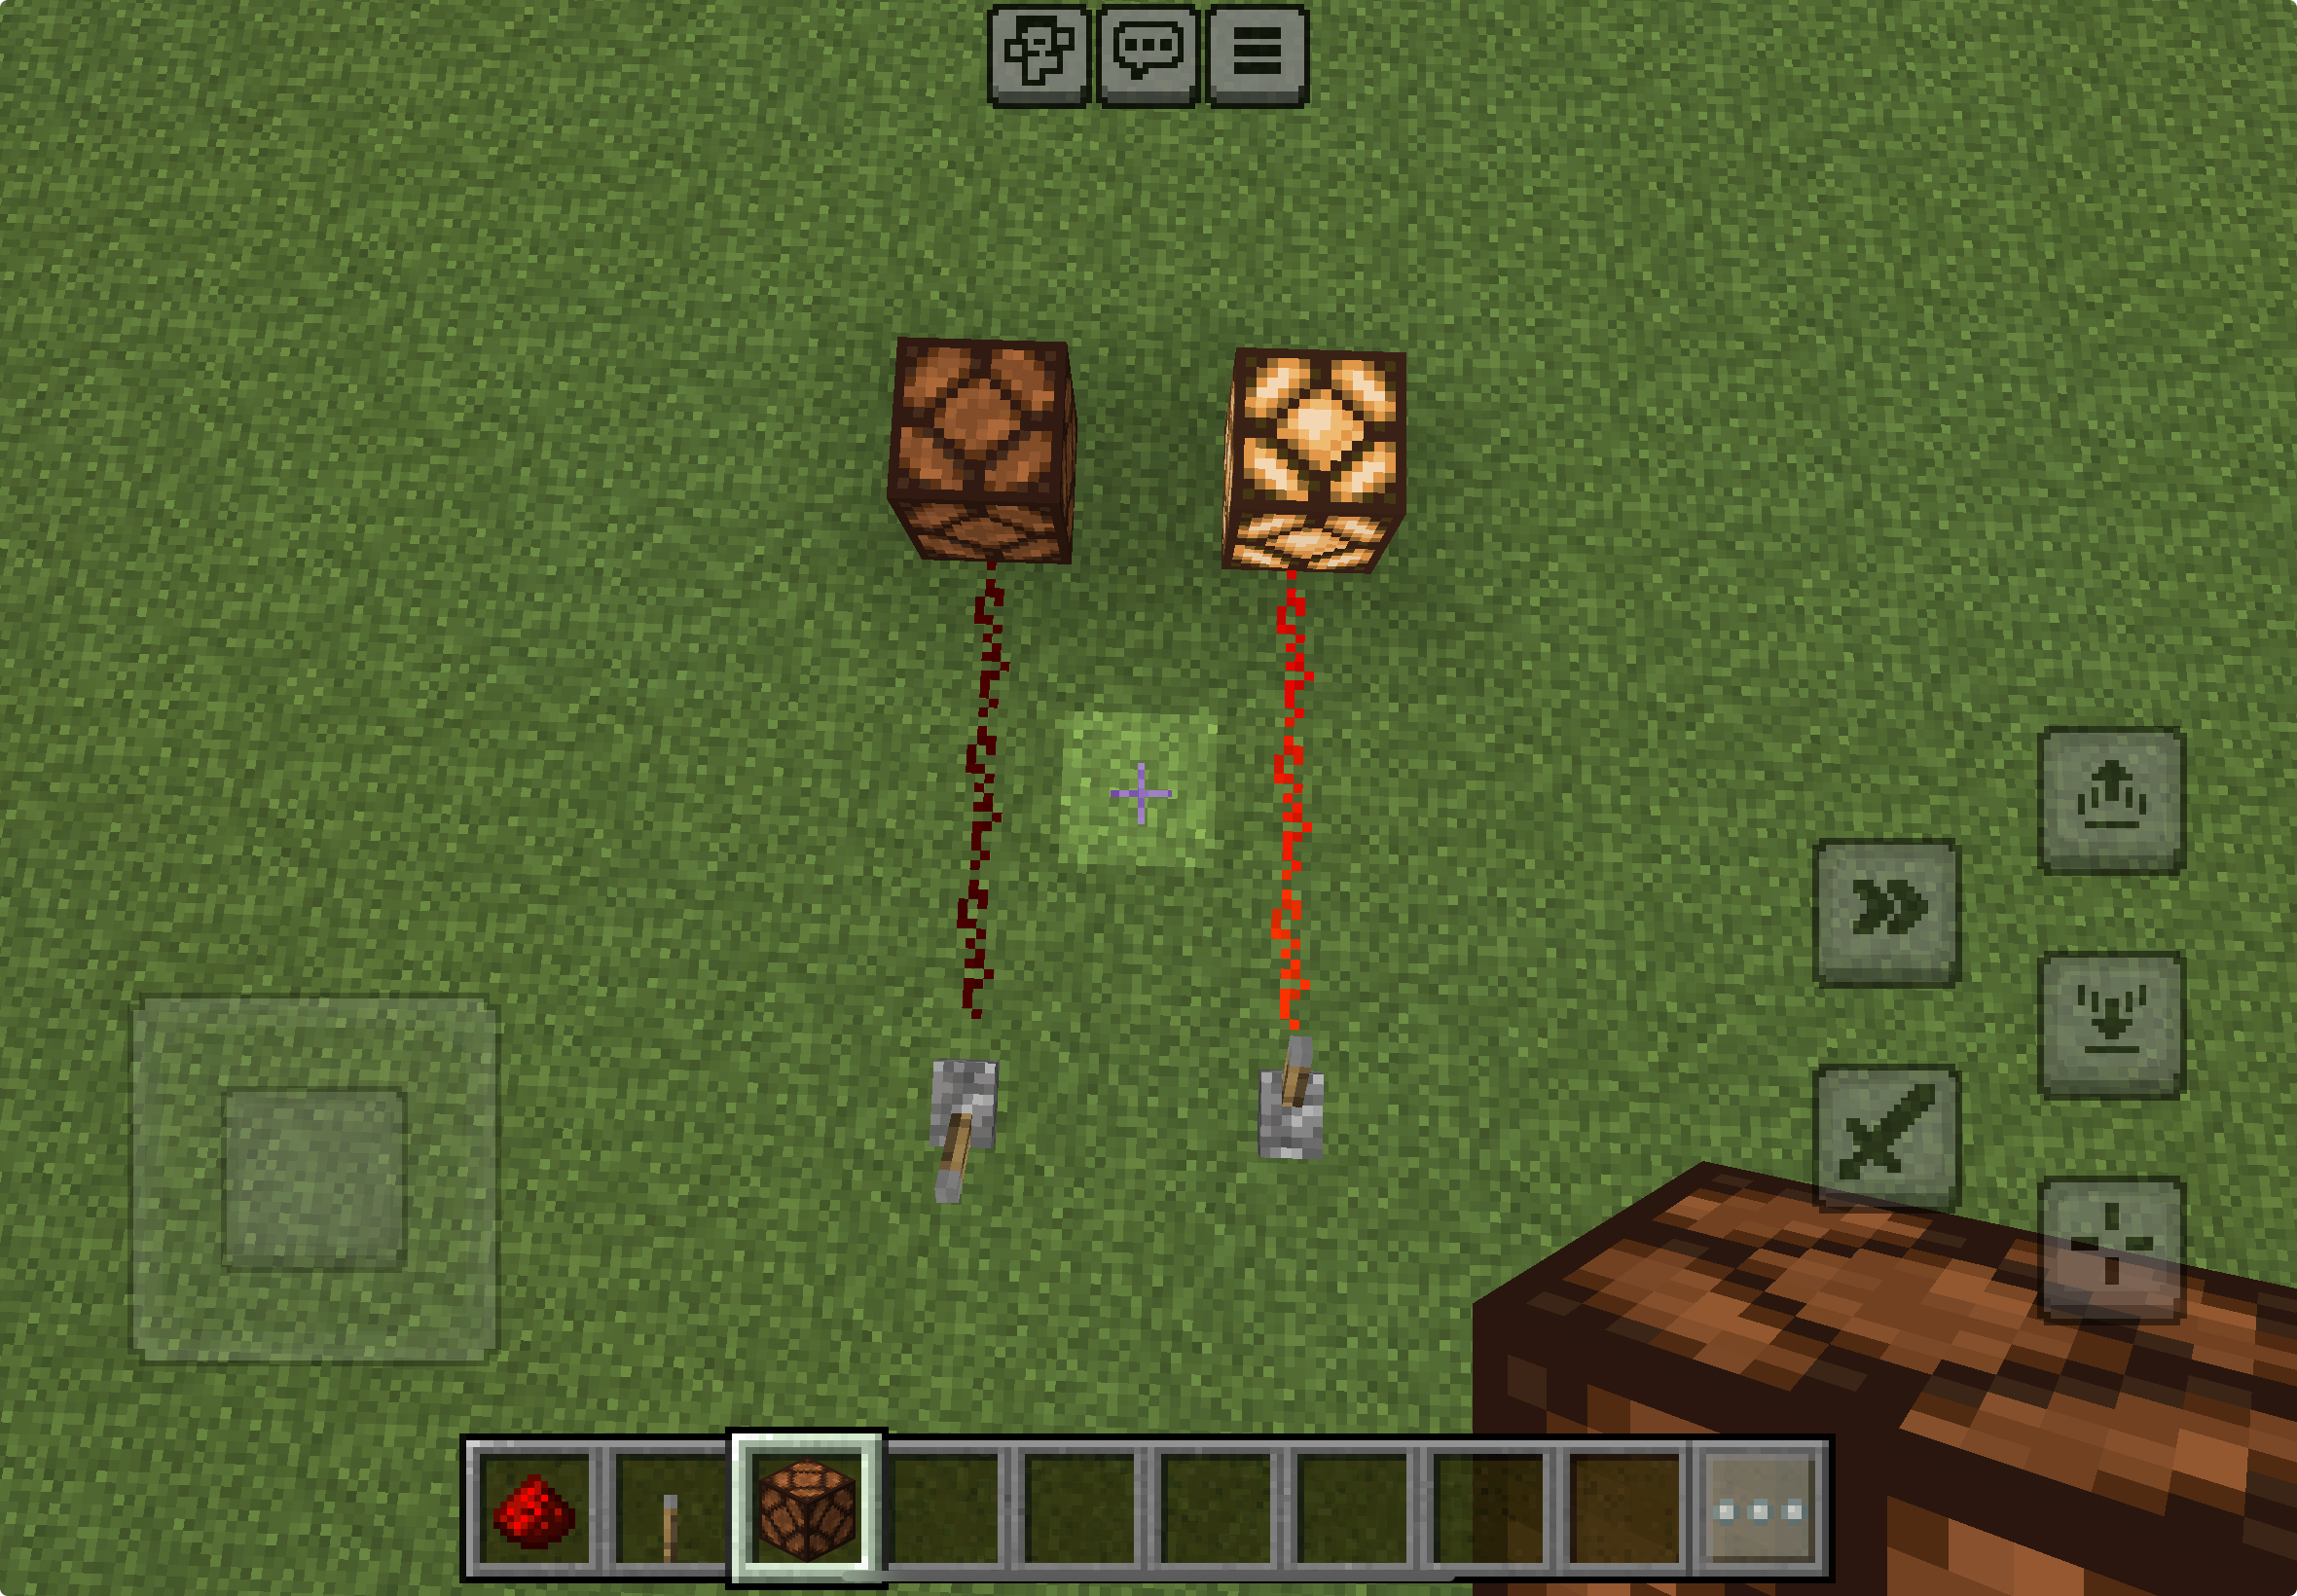
\includegraphics[width=0.6\textwidth]{images/zero_and_one_gate.png}
        \caption{Example of 0 and 1 in Minecraft Redstone Circuit}
    \end{figure}
\end{frame}

\begin{frame}{Basic Logic Gates}
    \begin{itemize}
        \item AND Gate: Output is 1 only when both inputs are 1
        \item OR Gate: Output is 1 when any input is 1
    \end{itemize}
\end{frame}

\begin{frame}{AND Gate in Minecraft}
    \begin{itemize}
        \item The AND gate outputs 1 only when both inputs are 1.
        \item In Minecraft, you can use redstone components to build an AND gate.
        \item Below are examples of different input combinations and their outputs:
    \end{itemize}
    \begin{figure}[ht]
        \centering
        \begin{minipage}{0.32\textwidth}
            \centering
            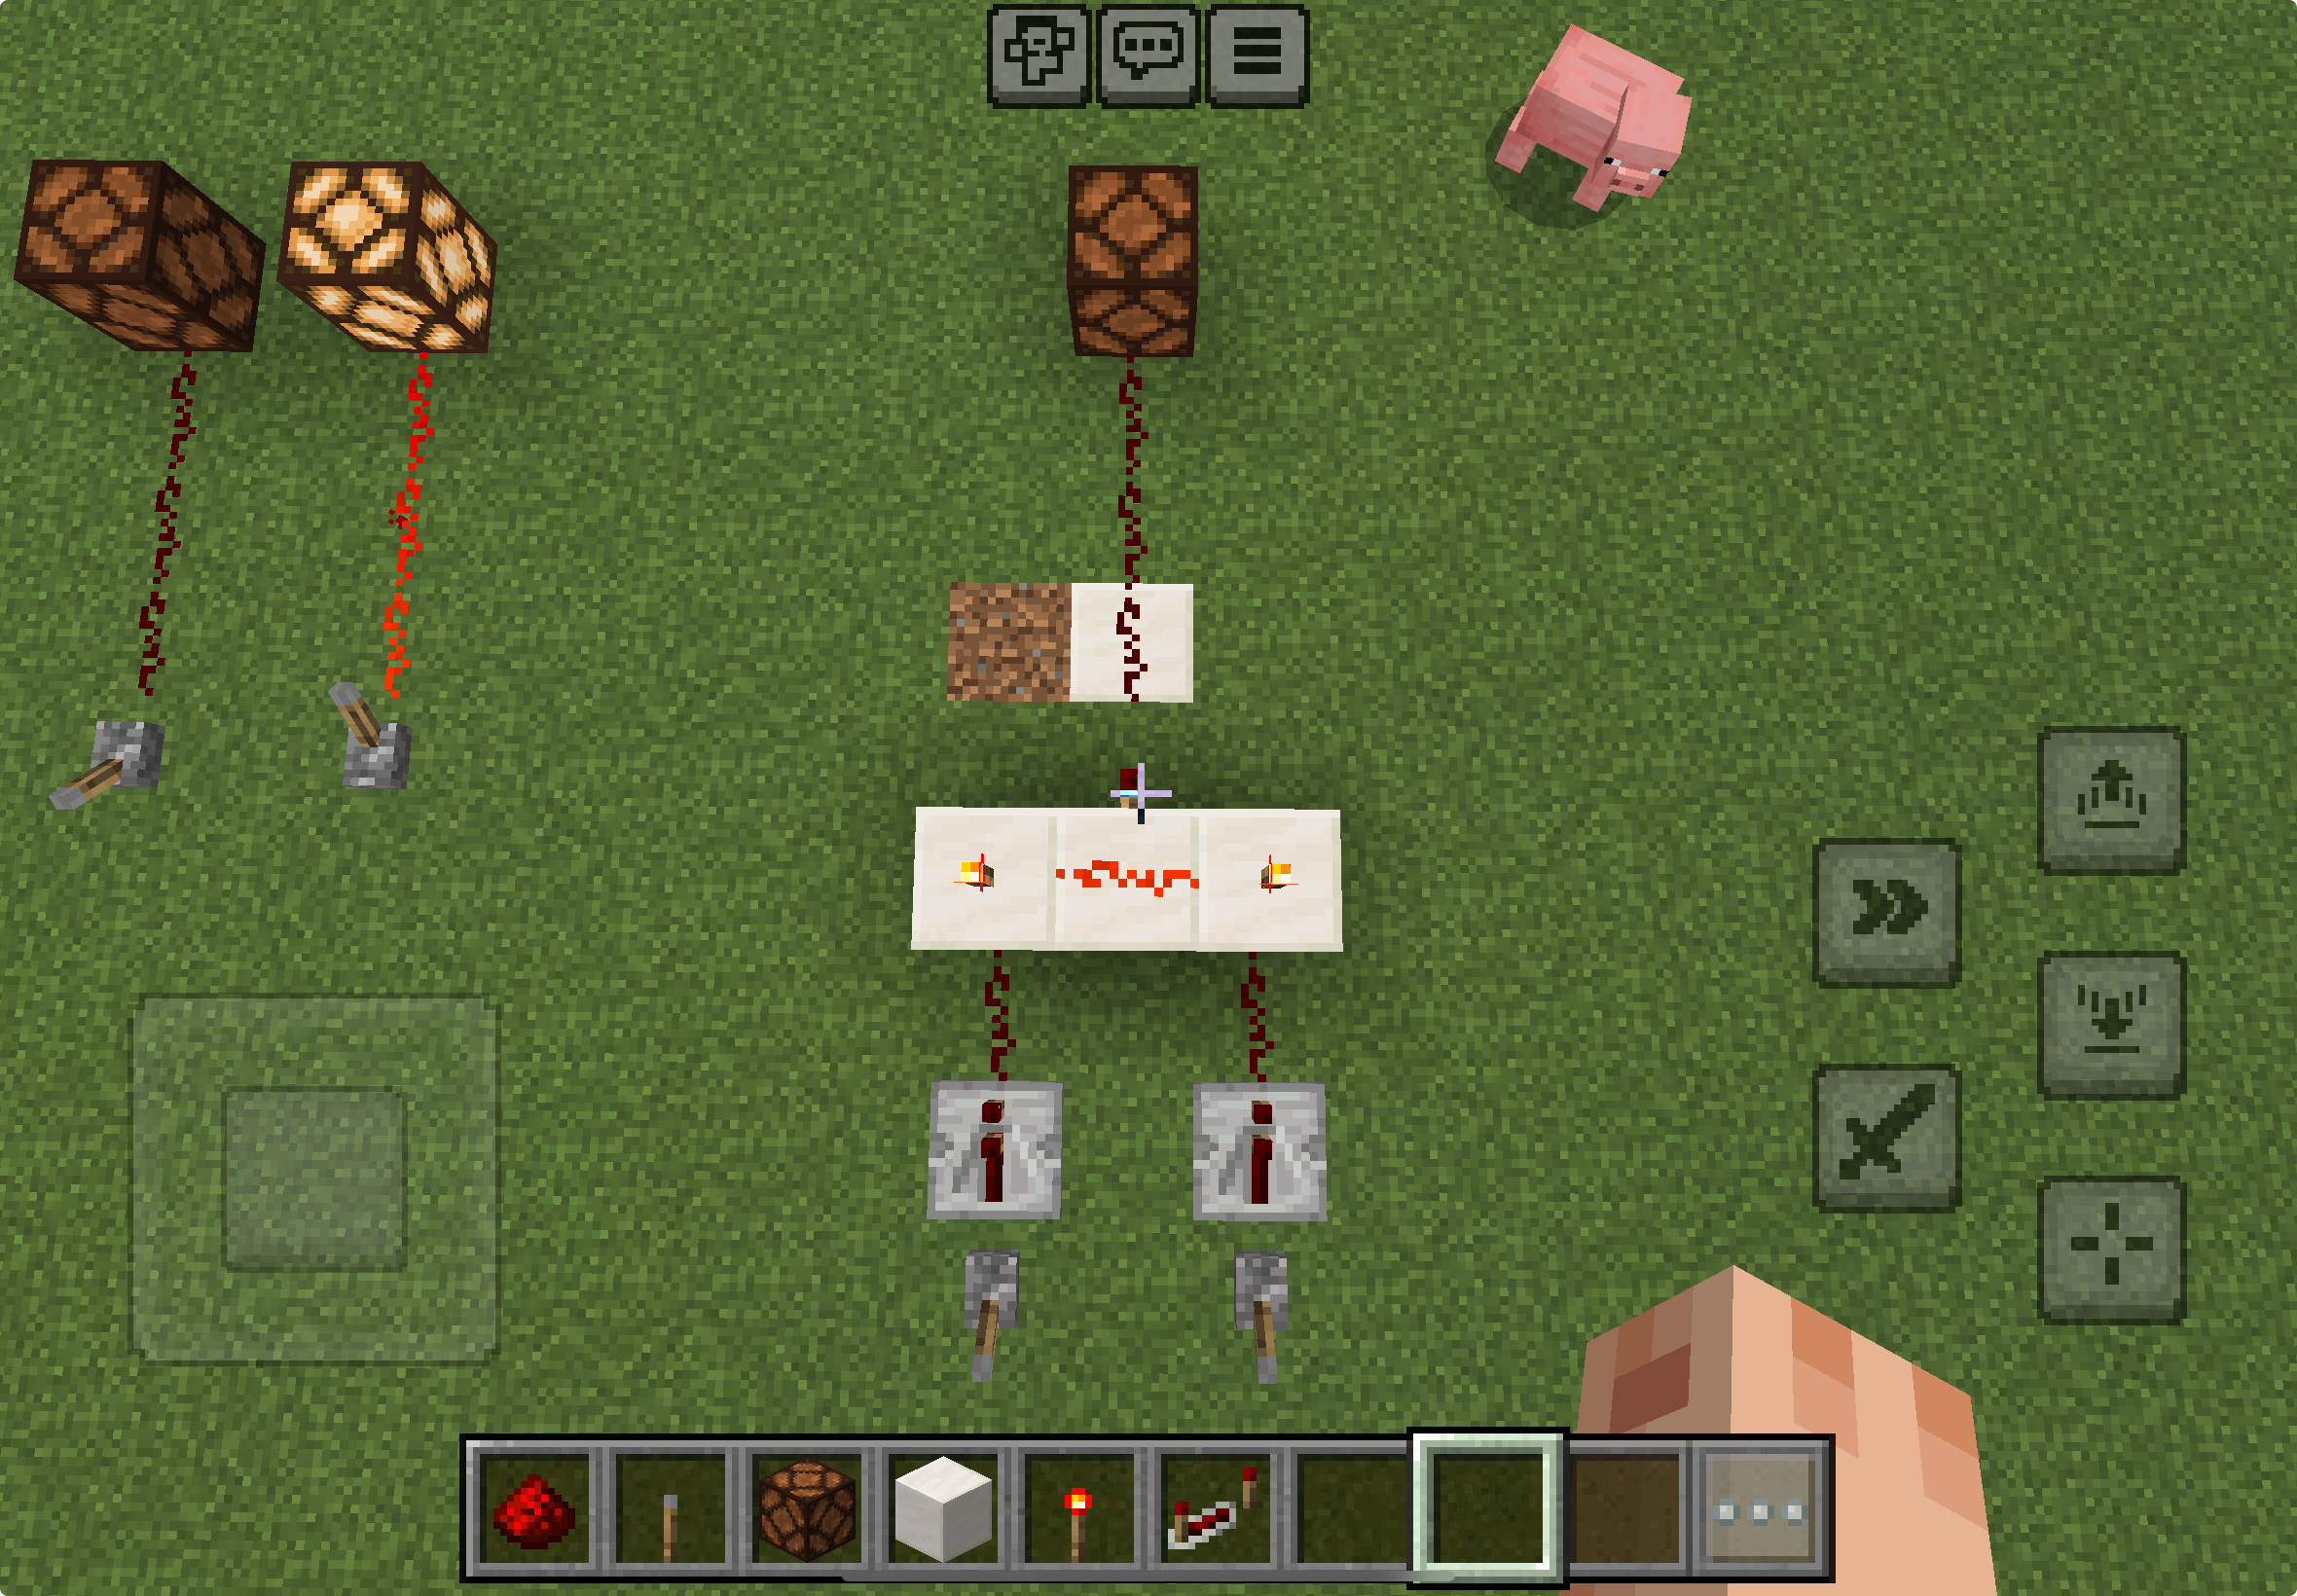
\includegraphics[width=\textwidth]{images/andgate_00.png}\\
            \small Input: 0, 0
        \end{minipage}
        \begin{minipage}{0.32\textwidth}
            \centering
            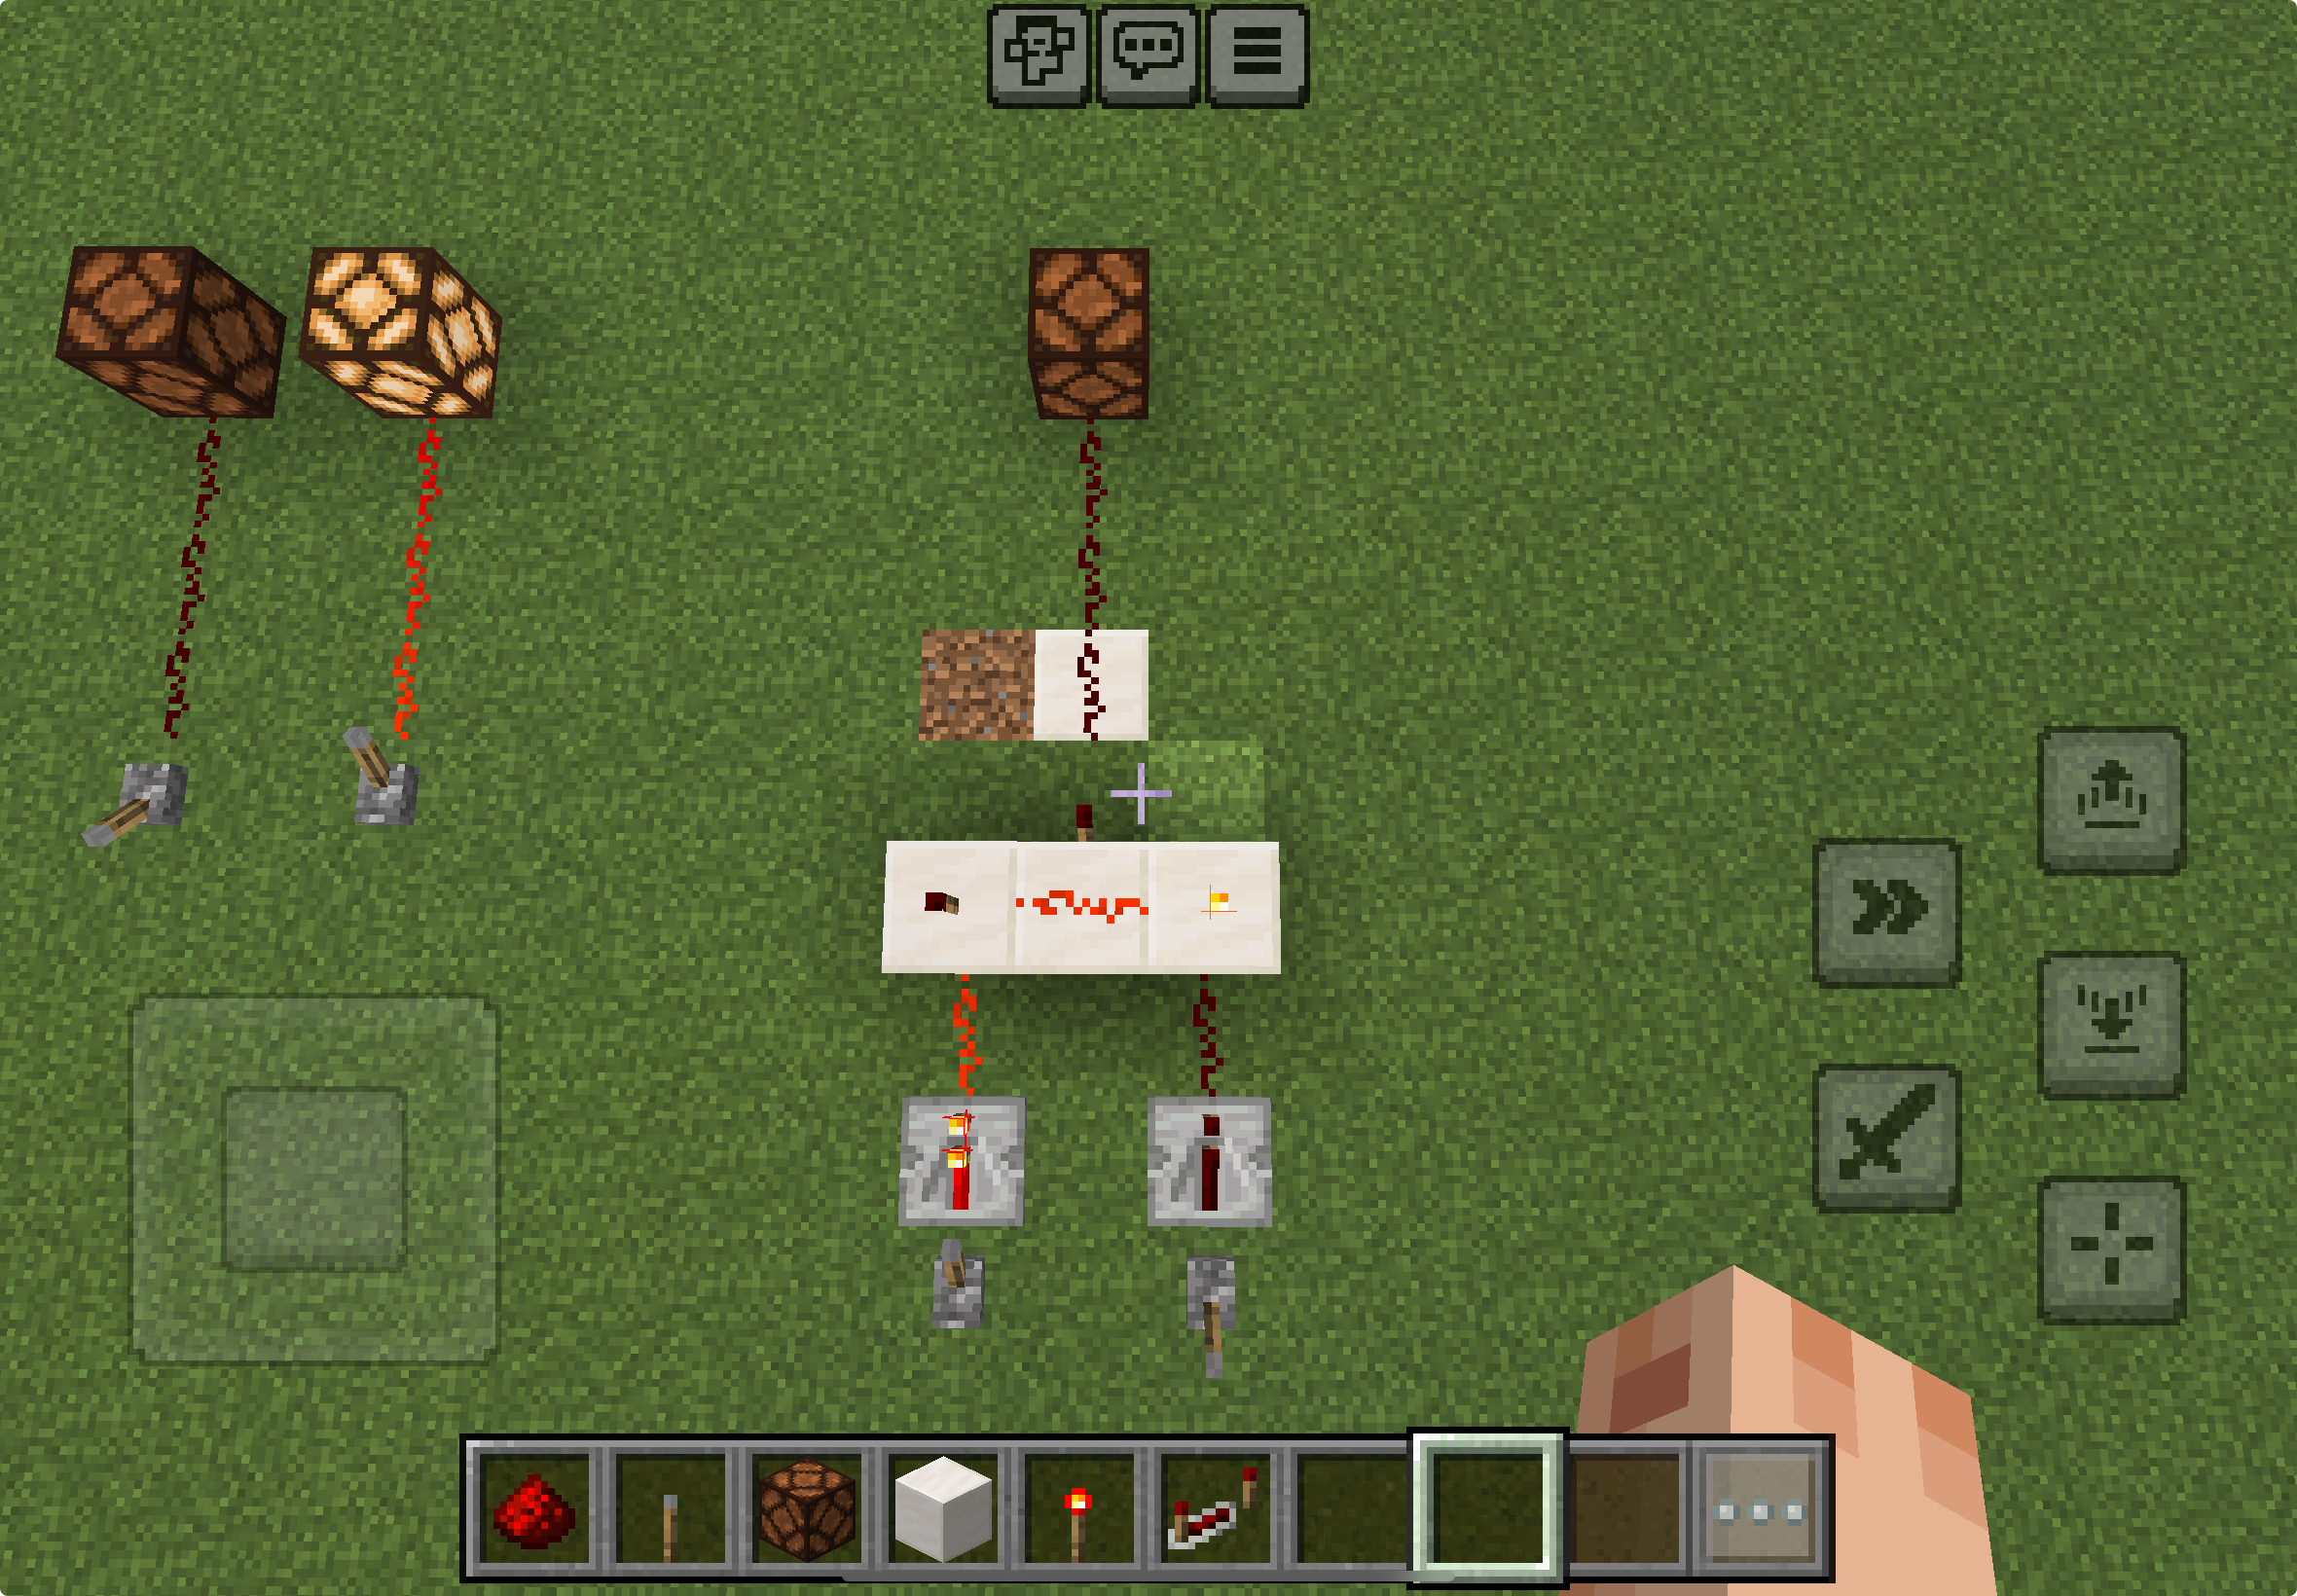
\includegraphics[width=\textwidth]{images/andgate_01.png}\\
            \small Input: 0, 1
        \end{minipage}
        \begin{minipage}{0.32\textwidth}
            \centering
            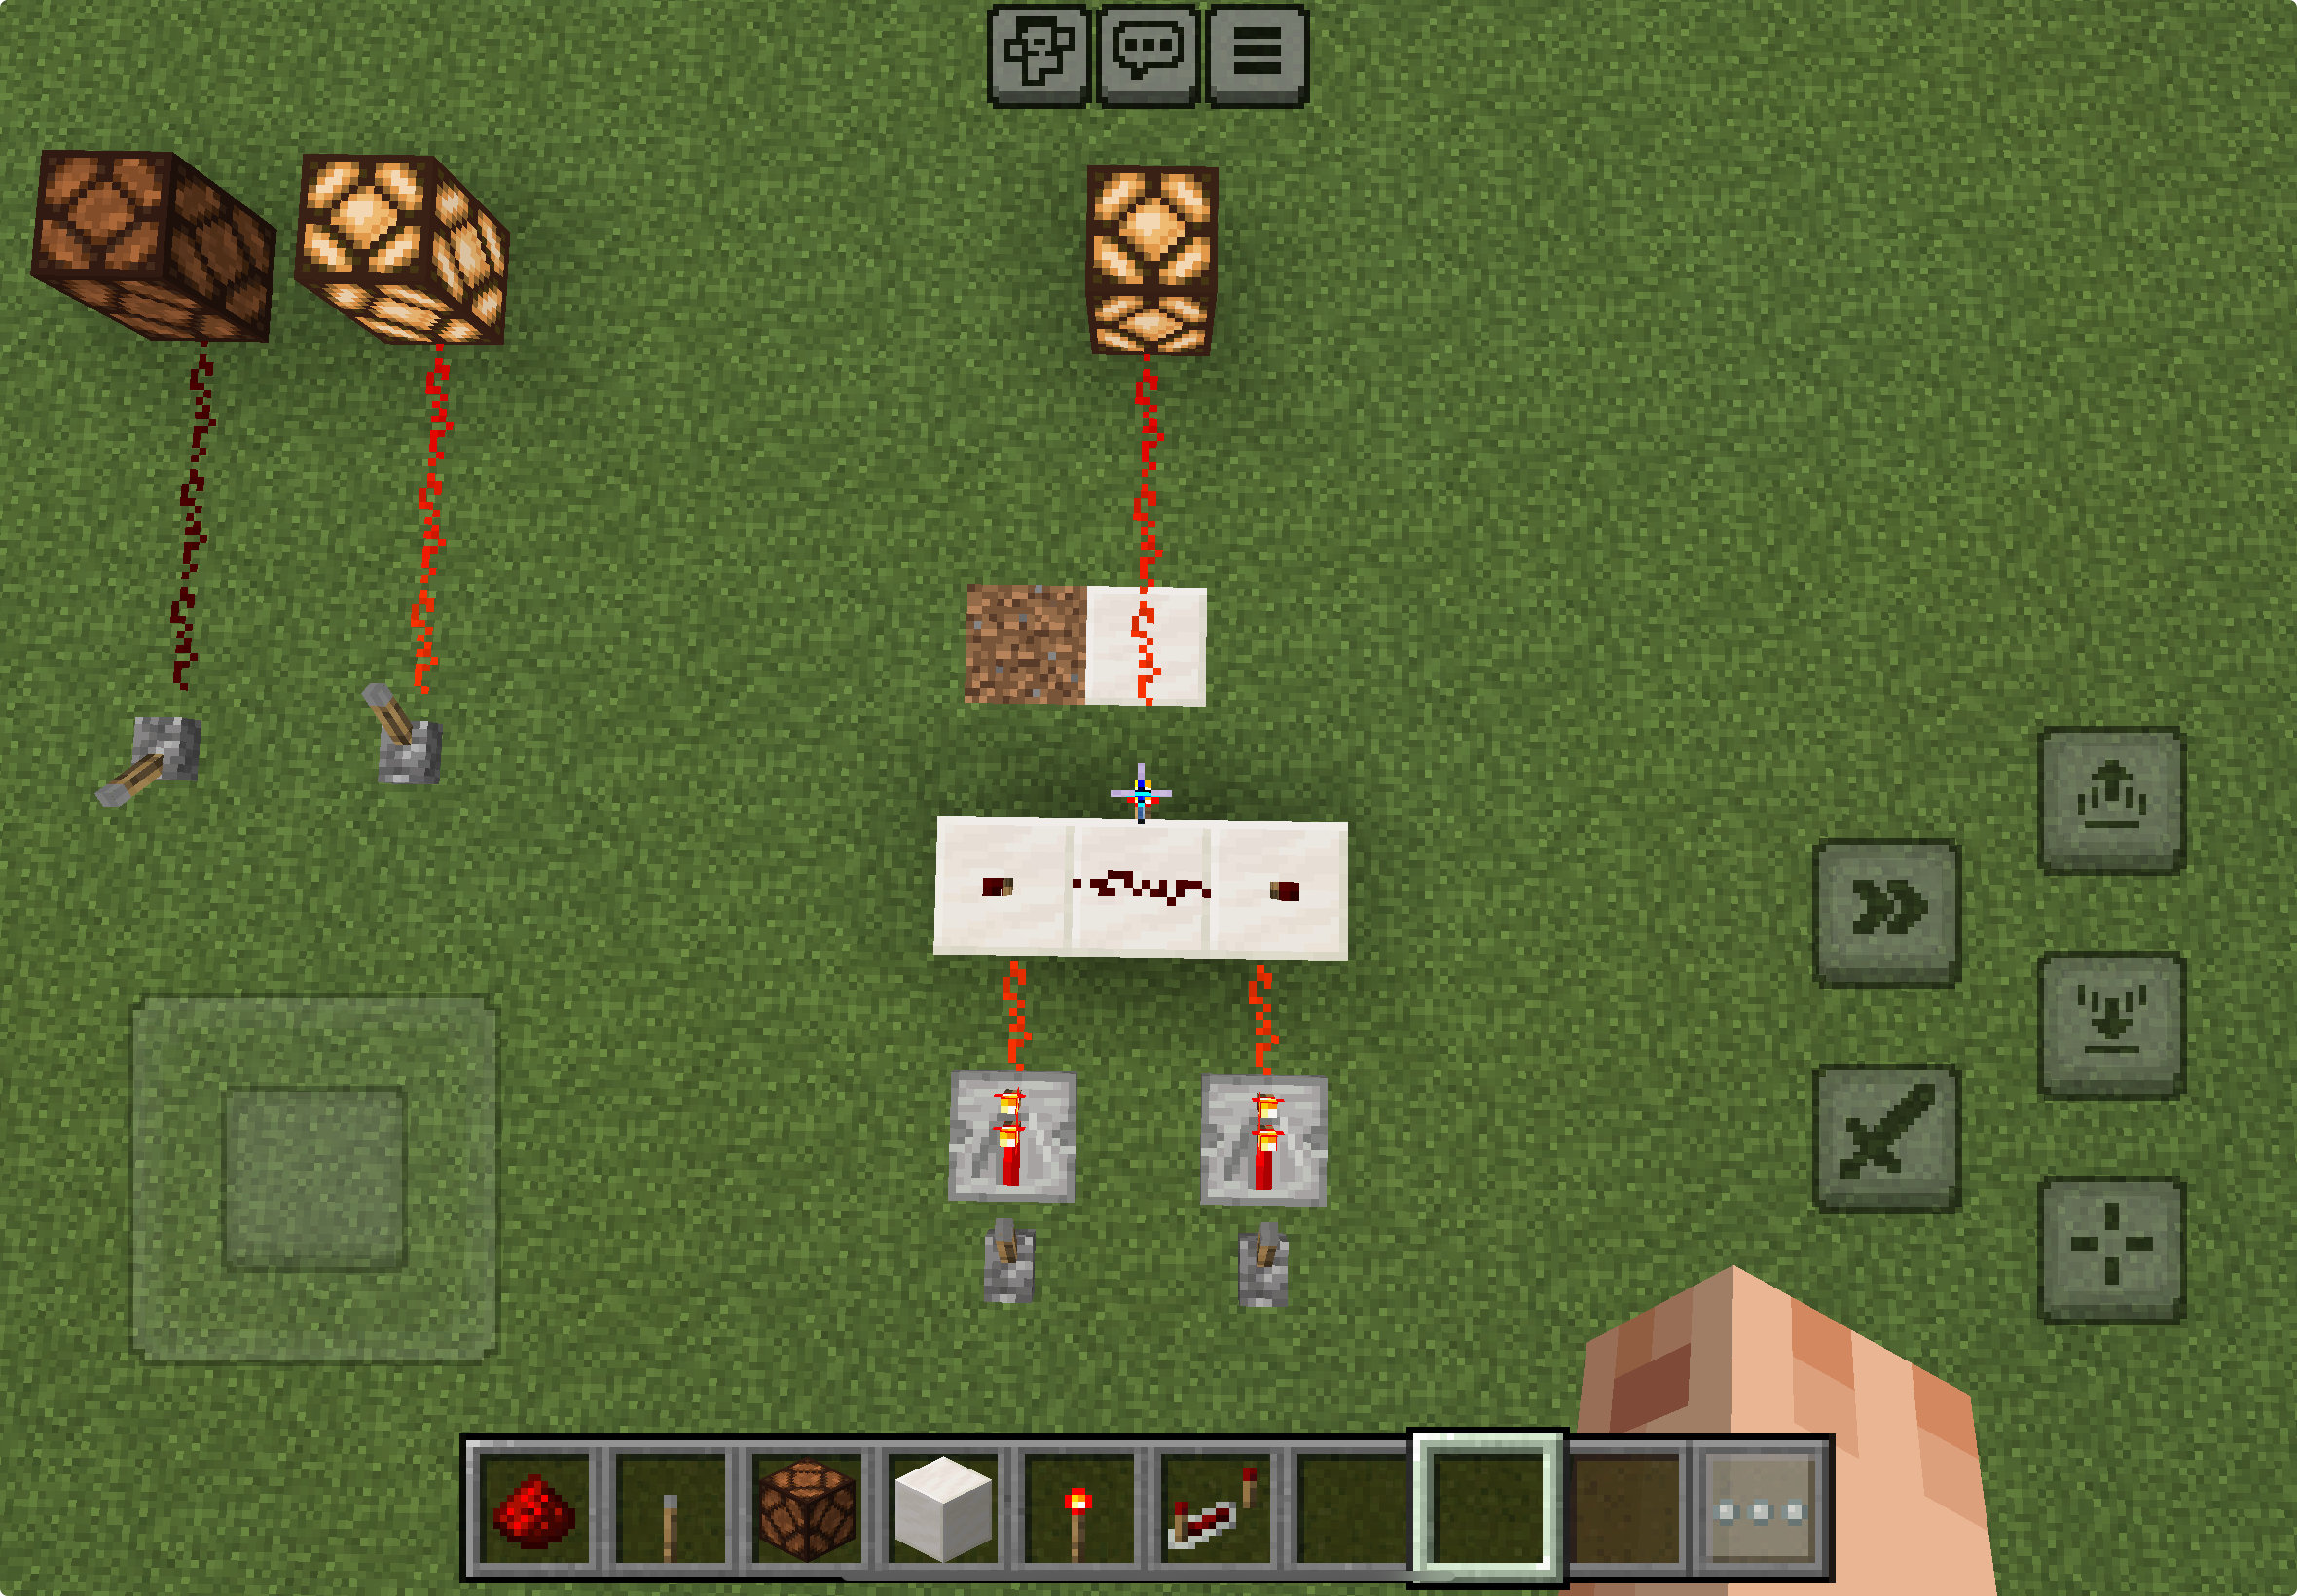
\includegraphics[width=\textwidth]{images/andgate_11.png}\\
            \small Input: 1, 1
        \end{minipage}
        \caption{AND Gate in Minecraft: Different Input Combinations}
    \end{figure}
\end{frame}

\begin{frame}{Logic Gate Truth Tables}
    \begin{block}{AND Gate}
        \begin{tabular}{|c|c|c|}
            \hline
            Input A & Input B & Output \\
            \hline
            0 & 0 & 0 \\
            0 & 1 & 0 \\
            1 & 0 & 0 \\
            1 & 1 & 1 \\
            \hline
        \end{tabular}
    \end{block}
\end{frame}


% OR gate 圖片與介紹頁
\begin{frame}{OR Gate in Minecraft}
    \begin{itemize}
        \item The OR gate outputs 1 when any input is 1.
        \item In Minecraft, you can use redstone to build an OR gate.
        \item Below are examples of different input combinations and their outputs:
    \end{itemize}
    \begin{figure}[ht]
        \centering
        \begin{minipage}{0.32\textwidth}
            \centering
            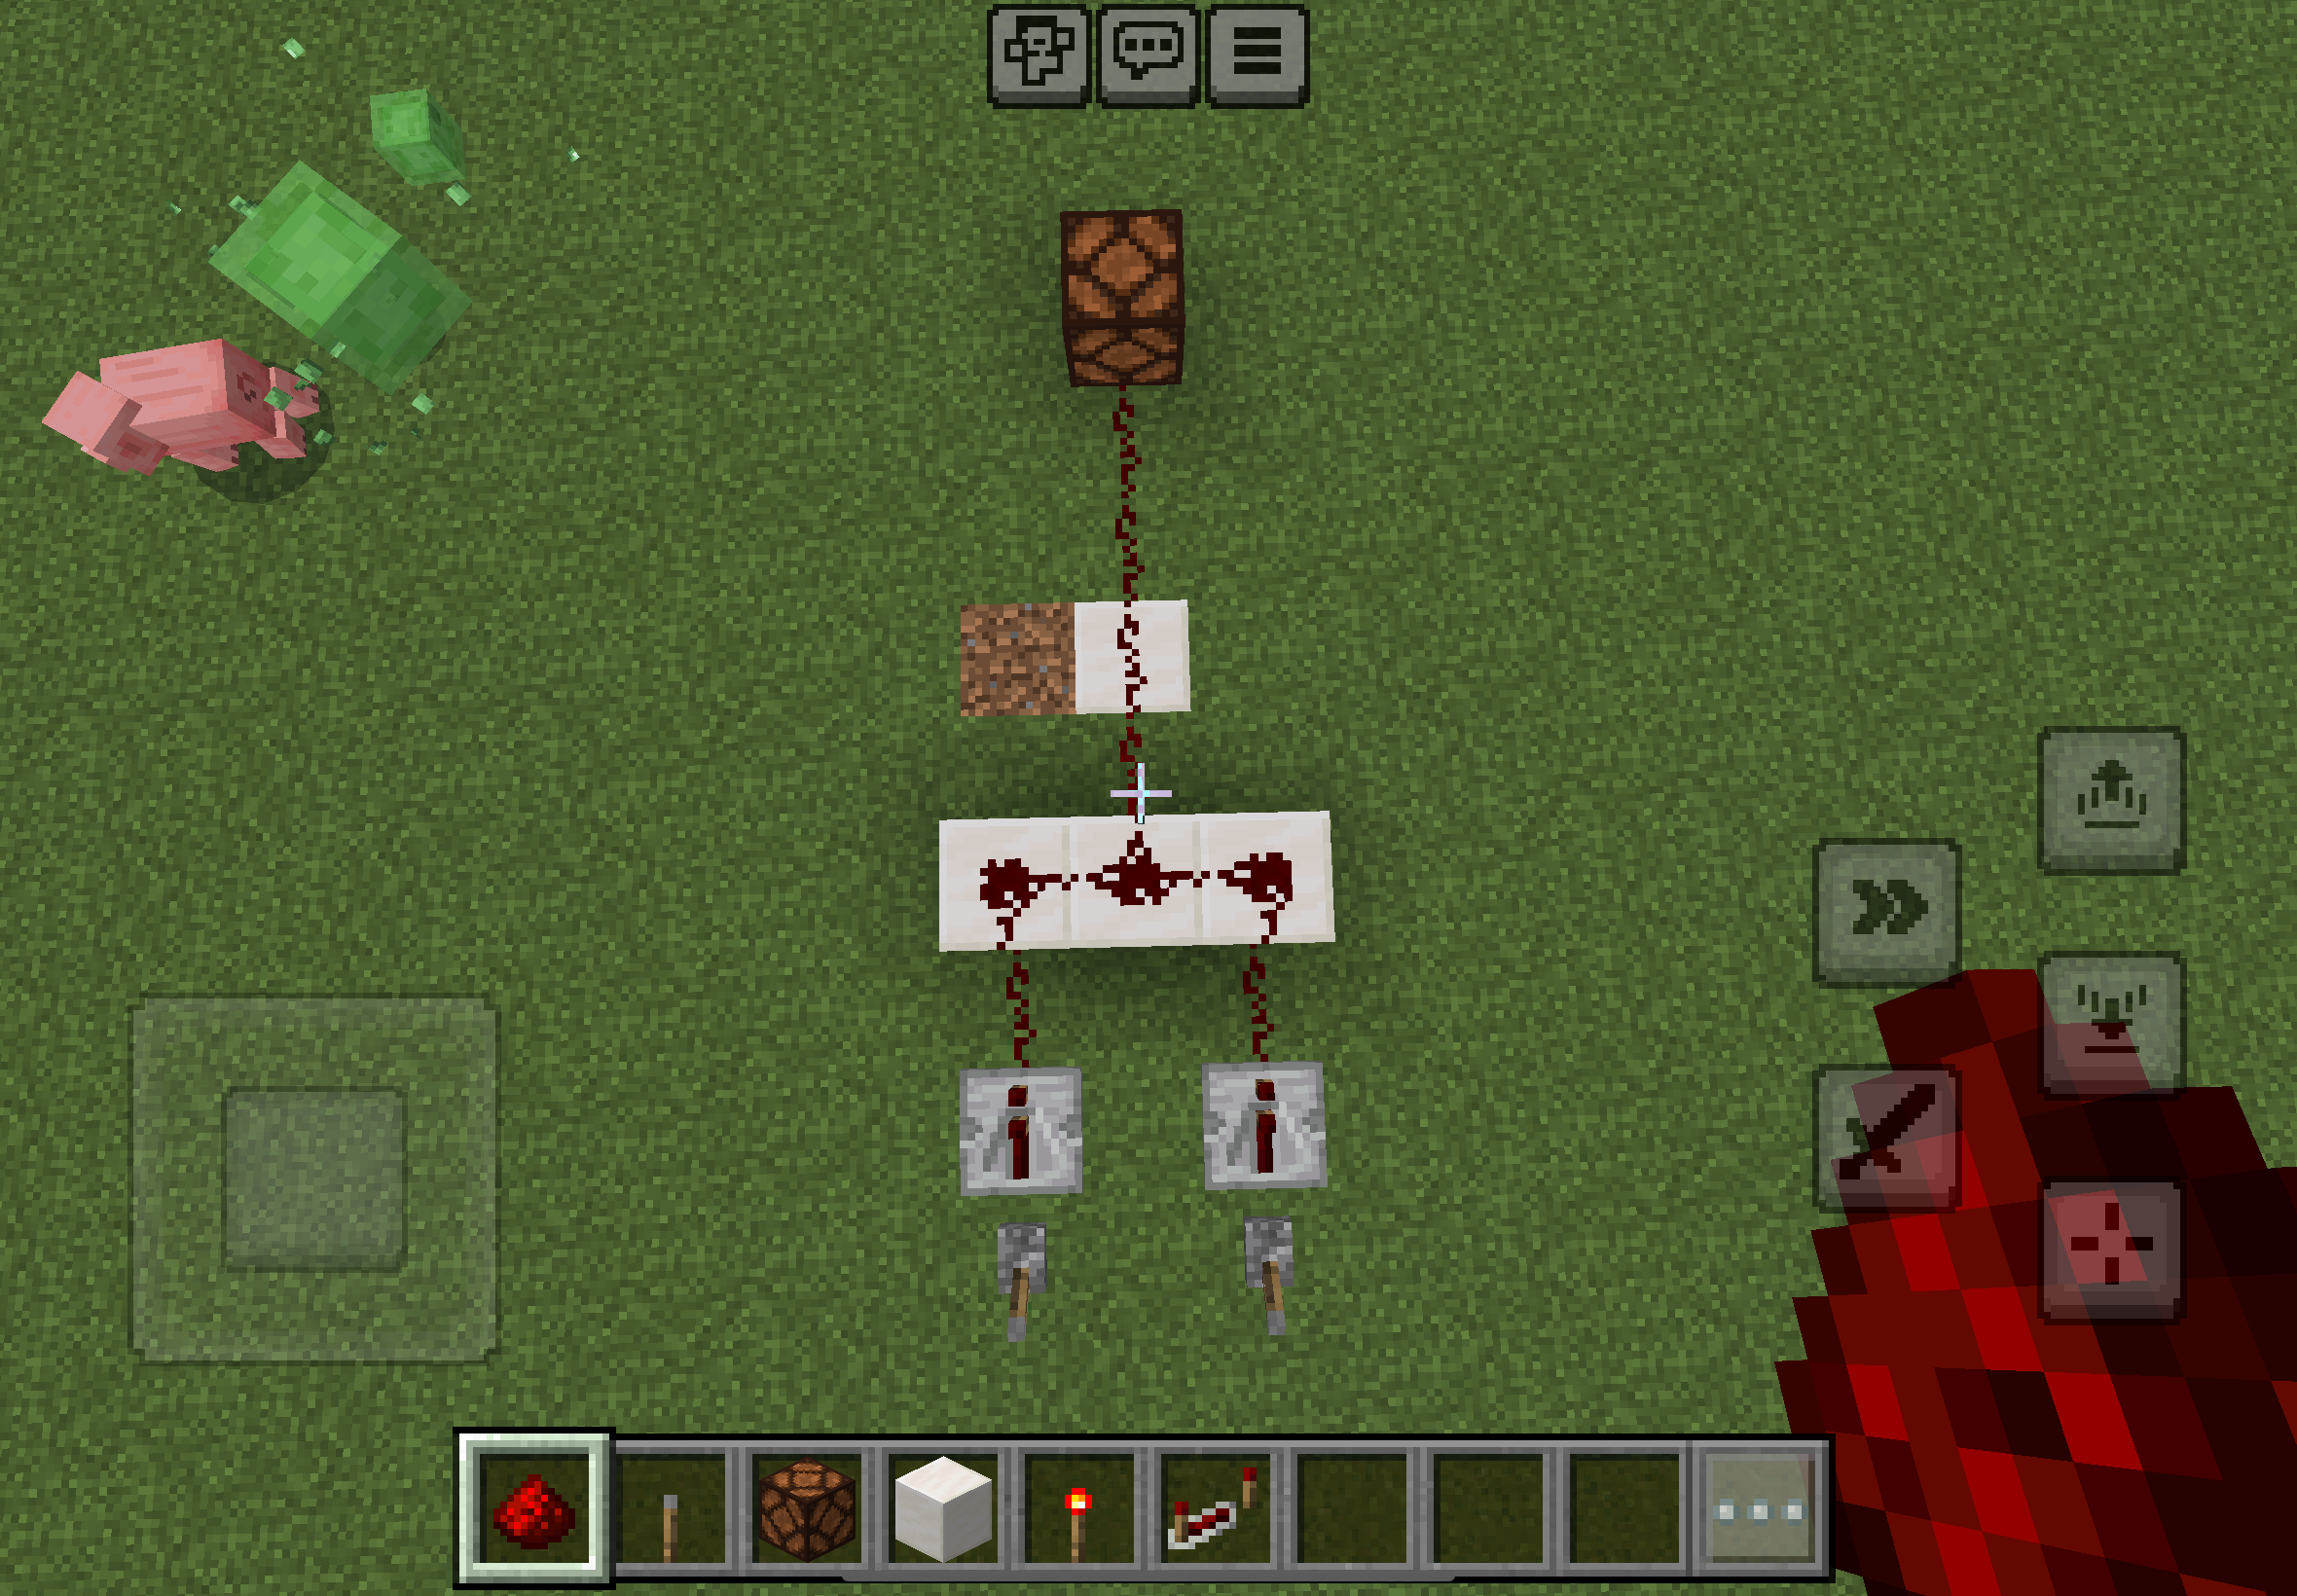
\includegraphics[width=\textwidth]{images/orgate_00.PNG}\\
            \small Input: 0, 0
        \end{minipage}
        \begin{minipage}{0.32\textwidth}
            \centering
            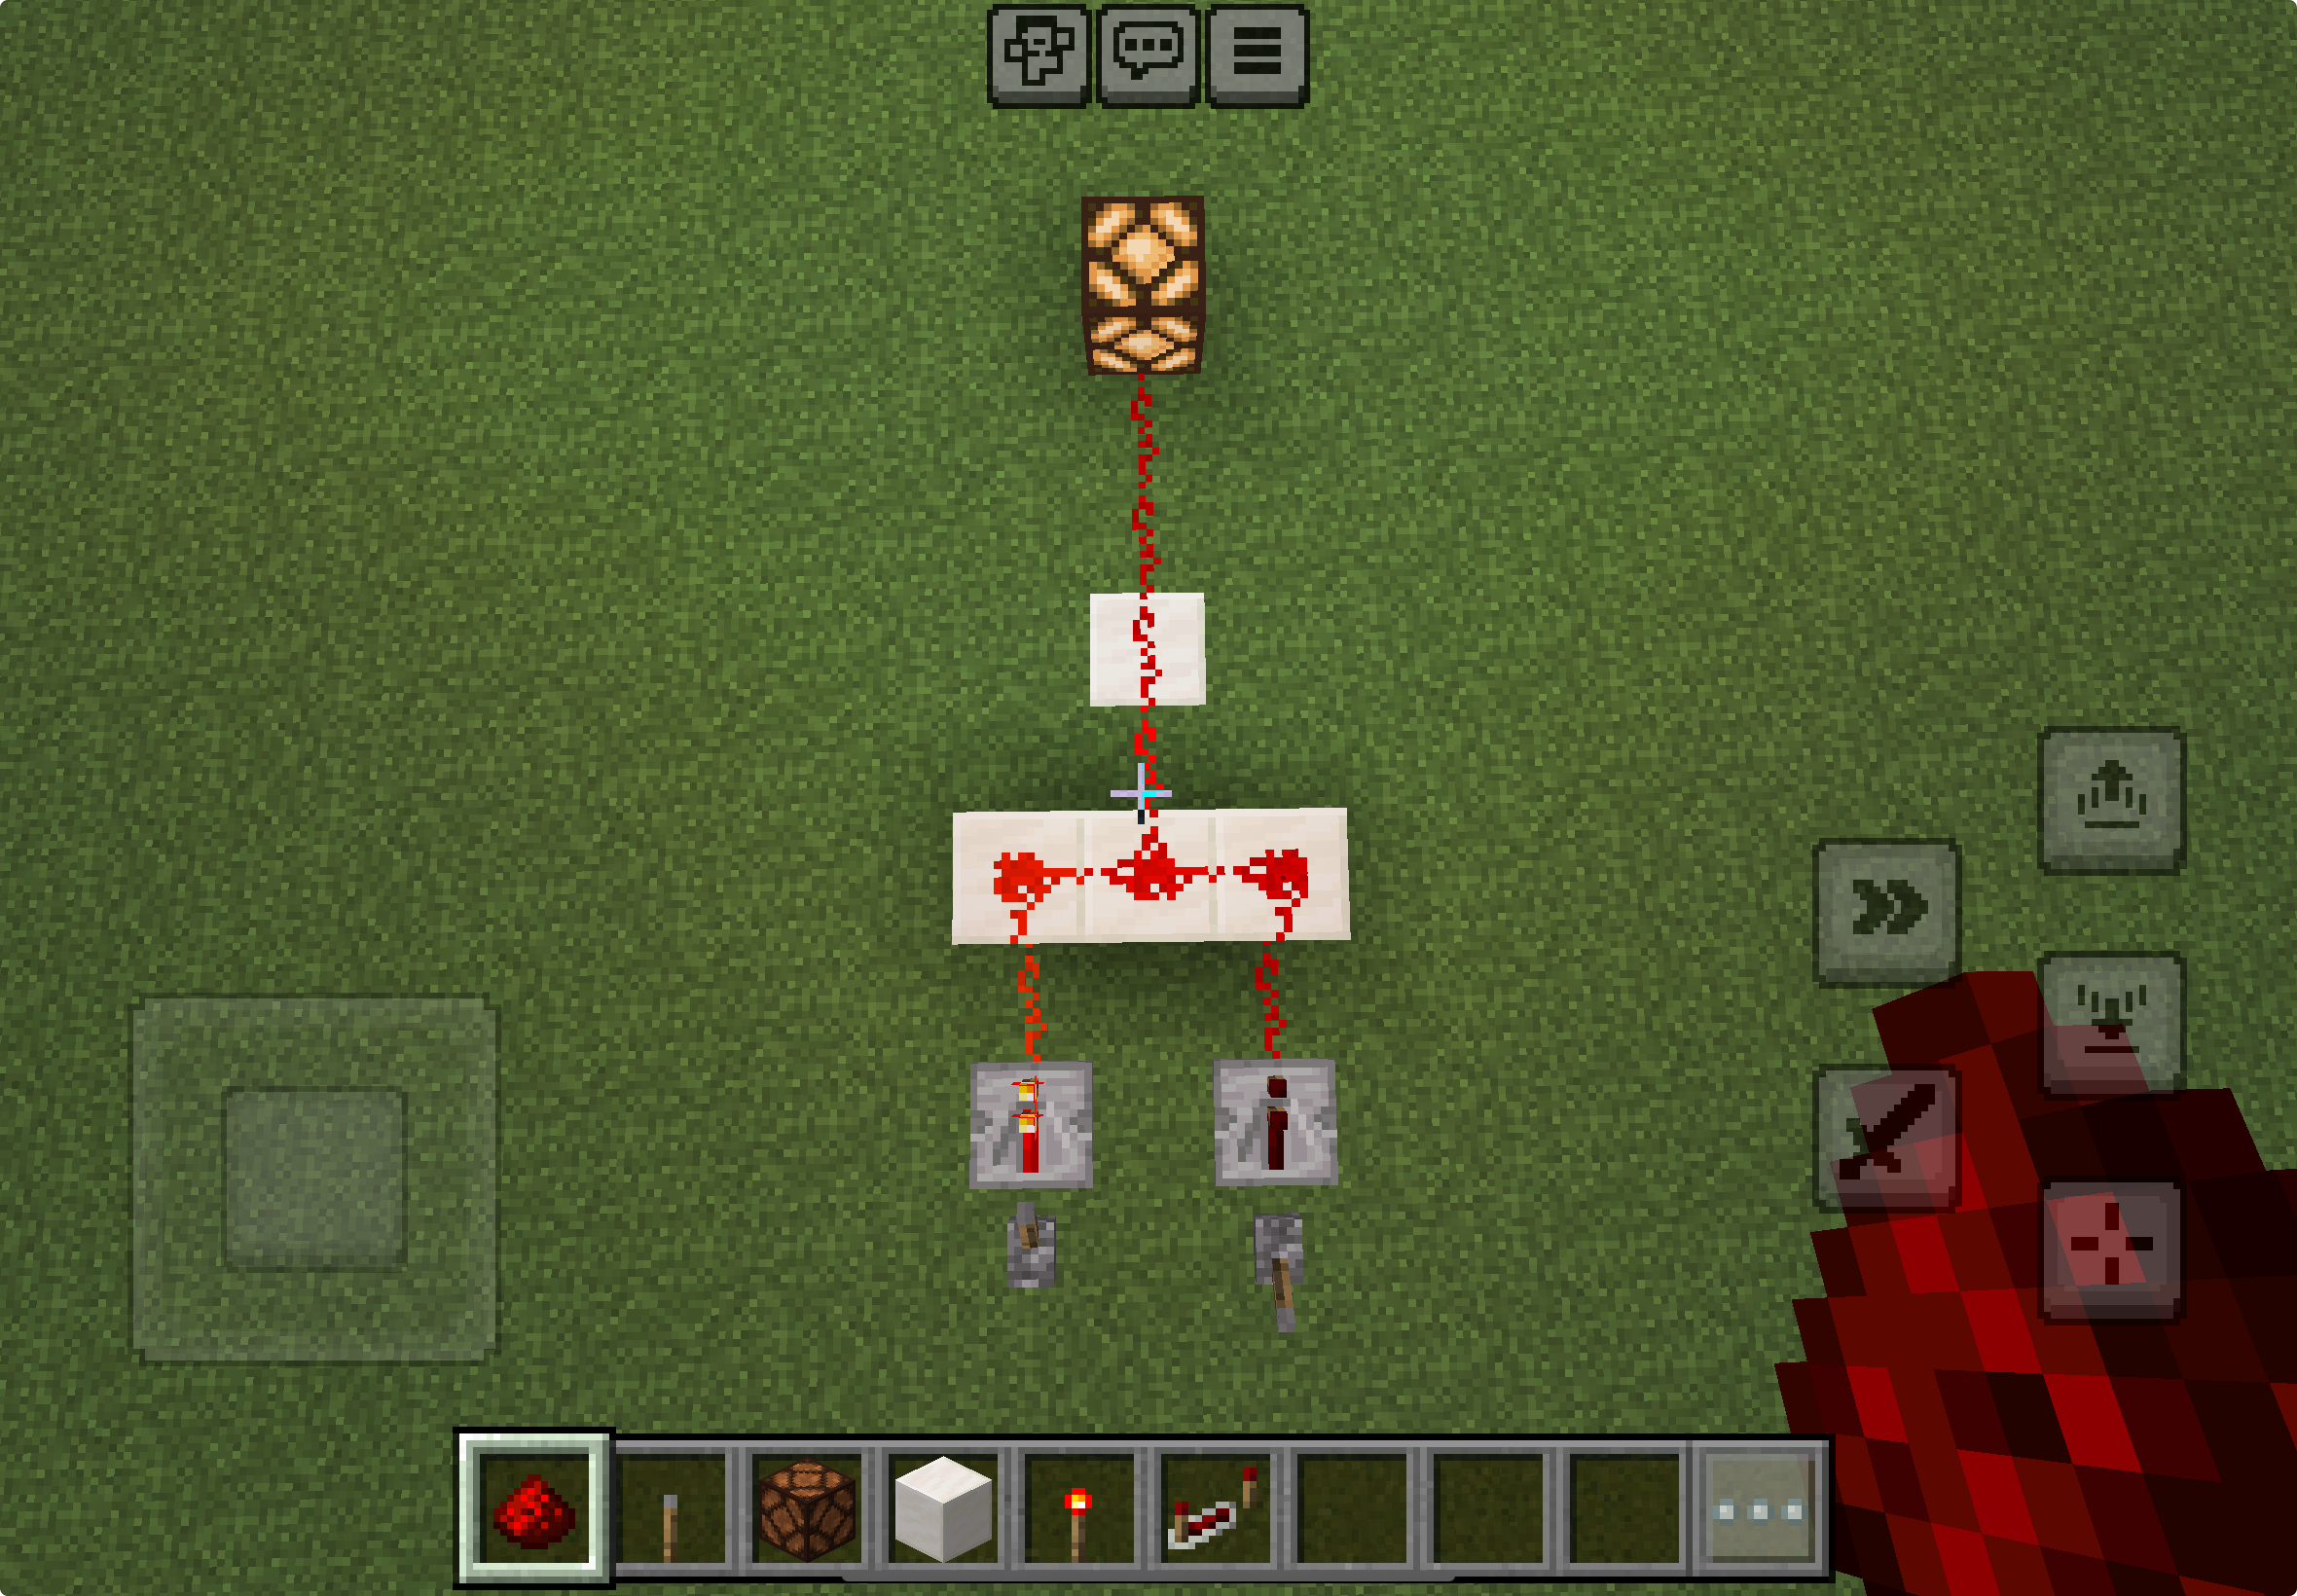
\includegraphics[width=\textwidth]{images/orgate_01.png}\\
            \small Input: 0, 1
        \end{minipage}
        \begin{minipage}{0.32\textwidth}
            \centering
            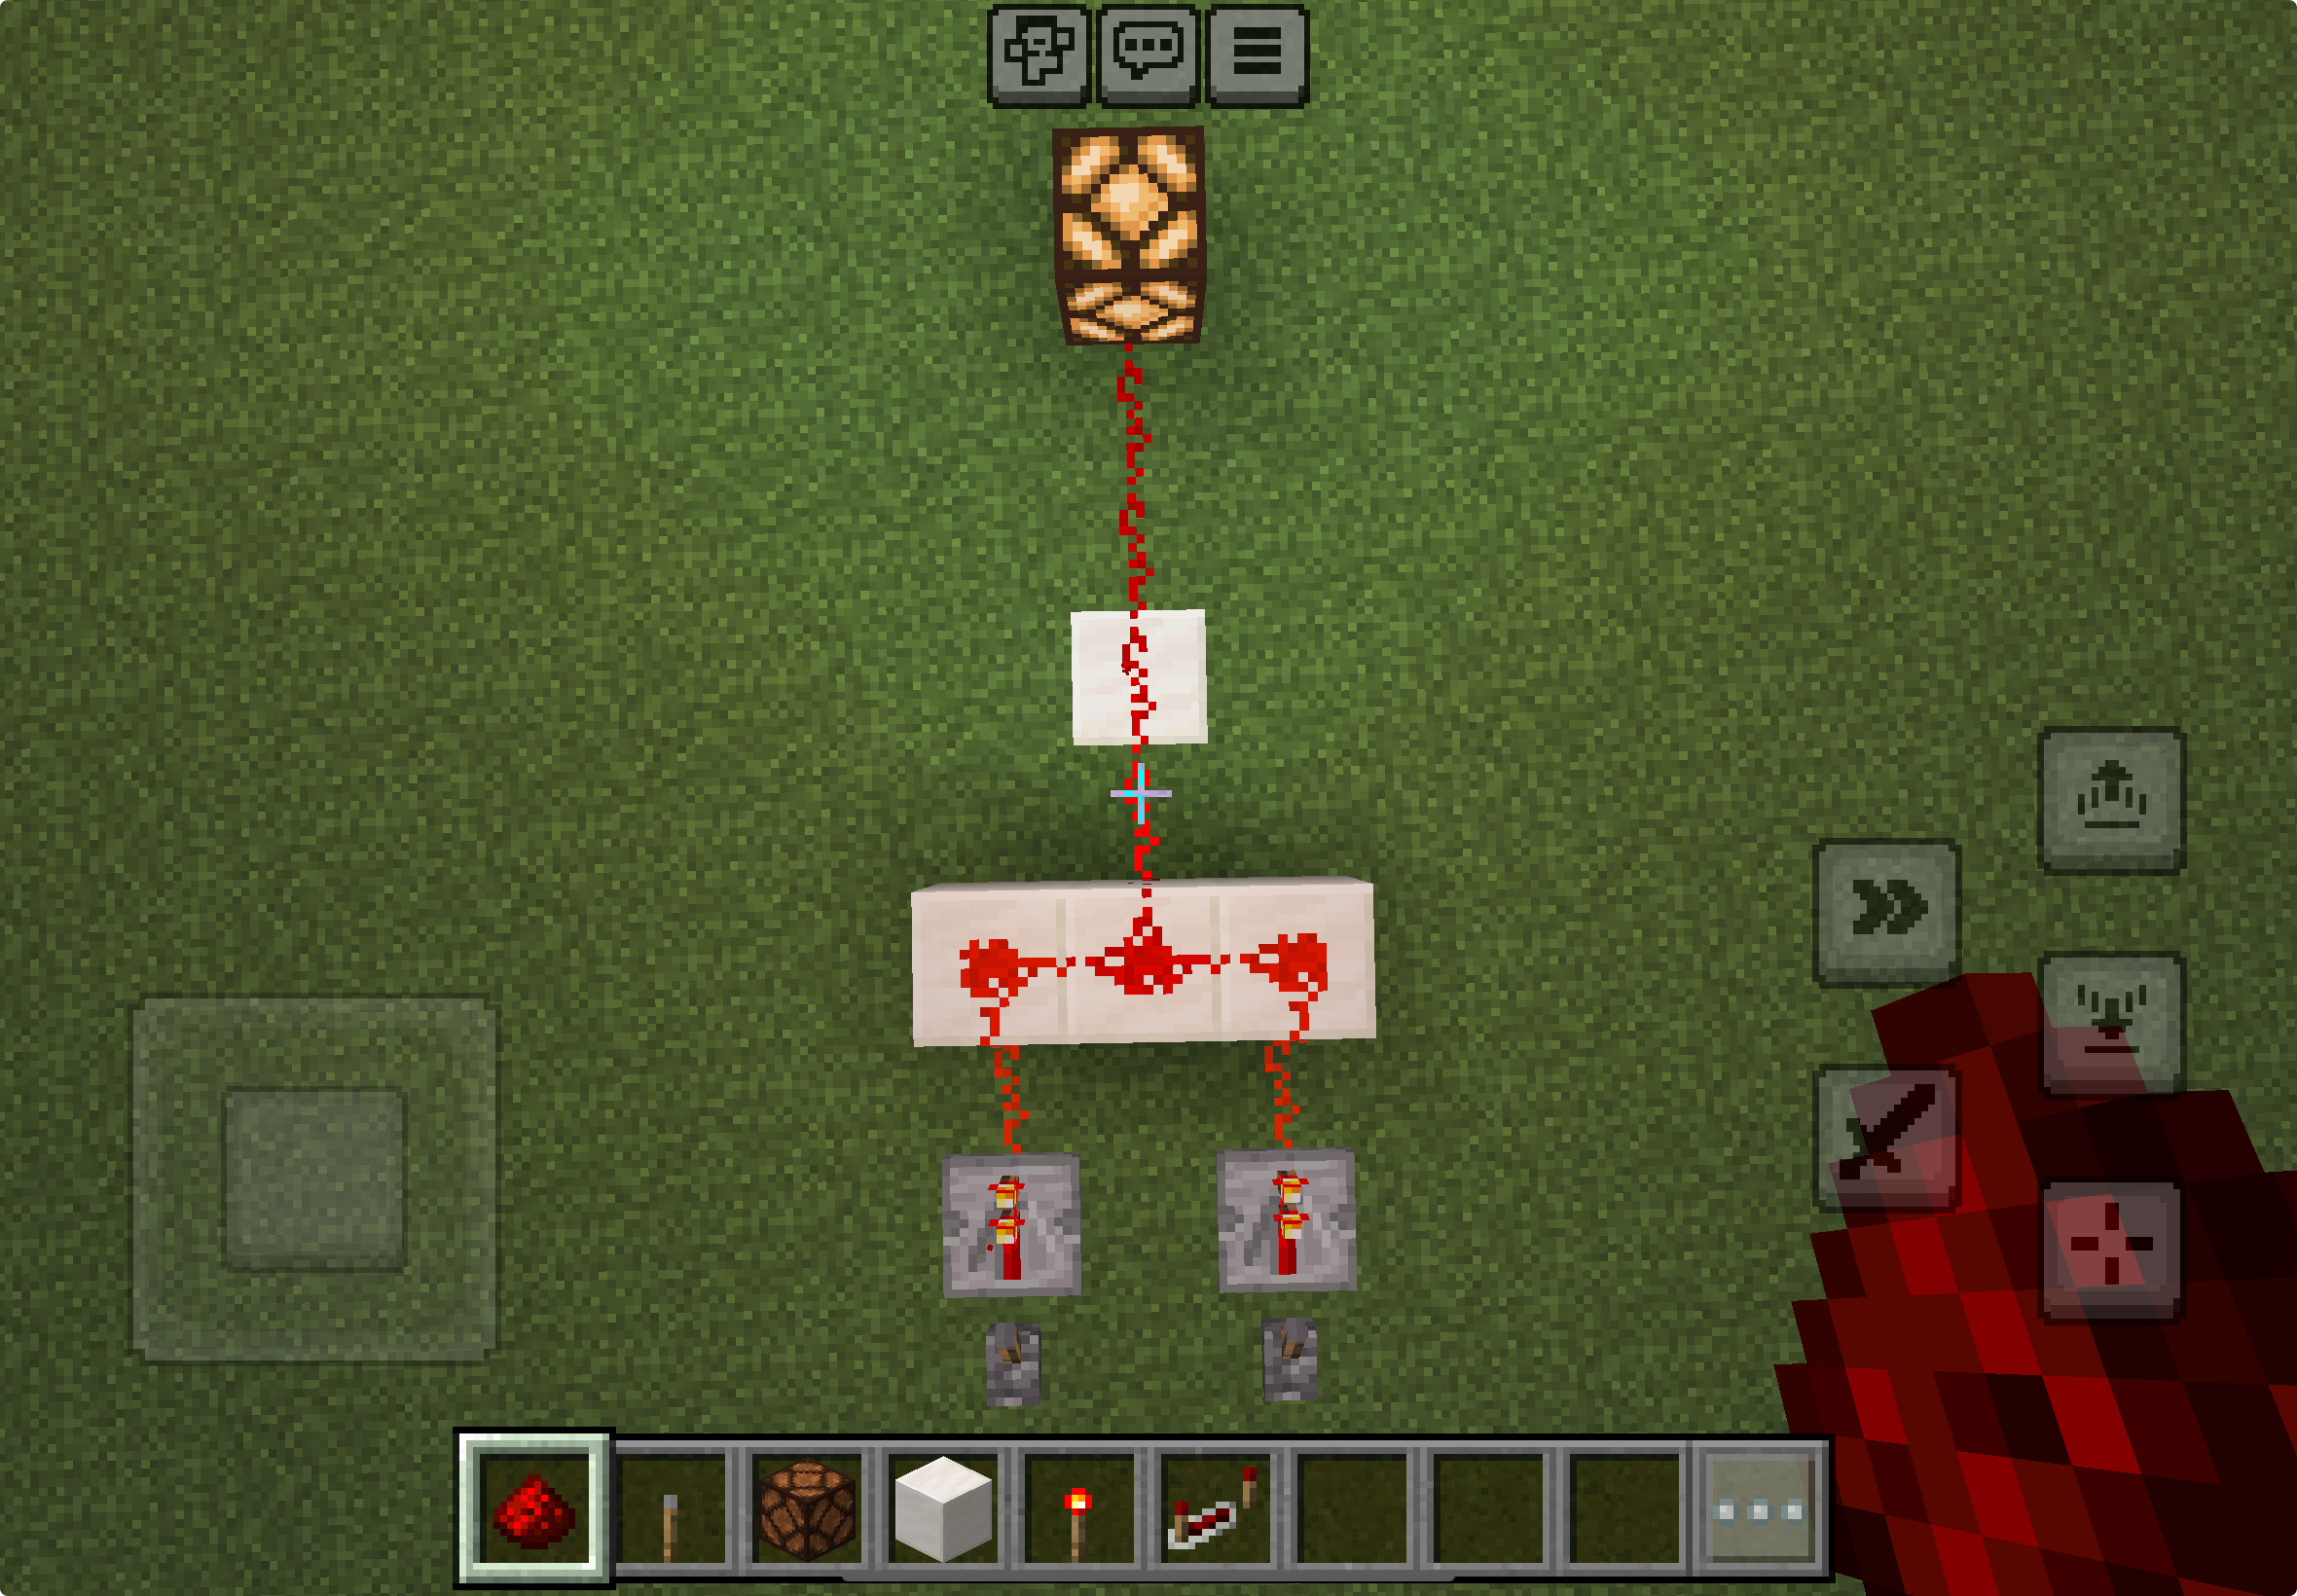
\includegraphics[width=\textwidth]{images/orgate_11.png}\\
            \small Input: 1, 1
        \end{minipage}
        \caption{OR Gate in Minecraft: Different Input Combinations}
    \end{figure}
\end{frame}

% OR gate truth table 獨立頁
\begin{frame}{Truth Table of OR Gate}
    \begin{block}{Truth Table}
        \begin{tabular}{|c|c|c|}
            \hline
            Input A & Input B & Output \\
            \hline
            0 & 0 & 0 \\
            0 & 1 & 1 \\
            1 & 0 & 1 \\
            1 & 1 & 1 \\
            \hline
        \end{tabular}
    \end{block}
\end{frame}

% XOR gate 圖片與介紹頁
\begin{frame}{XOR Gate in Minecraft}
    \begin{itemize}
        \item The XOR (exclusive OR) gate outputs 1 only when the two inputs are different.
        \item In Minecraft, you can use redstone to build an XOR gate.
        \item Below are examples of different input combinations and their outputs:
    \end{itemize}
    \begin{figure}[ht]
        \centering
        \begin{minipage}{0.24\textwidth}
            \centering
            \includegraphics[width=\textwidth]{images/xorgate_00.png}\\
            \small Input: 0, 0
        \end{minipage}
        \begin{minipage}{0.24\textwidth}
            \centering
            \includegraphics[width=\textwidth]{images/xorgate_01.png}\\
            \small Input: 0, 1
        \end{minipage}
        \begin{minipage}{0.24\textwidth}
            \centering
            \includegraphics[width=\textwidth]{images/xorgate_10.png}\\
            \small Input: 1, 0
        \end{minipage}
        \begin{minipage}{0.24\textwidth}
            \centering
            \includegraphics[width=\textwidth]{images/xorgate_11.png}\\
            \small Input: 1, 1
        \end{minipage}
        \caption{XOR Gate in Minecraft: Different Input Combinations}
    \end{figure}
\end{frame}

% XOR gate truth table 獨立頁
\begin{frame}{Truth Table of XOR Gate}
    \begin{block}{Truth Table}
        \begin{tabular}{|c|c|c|}
            \hline
            Input A & Input B & Output \\
            \hline
            0 & 0 & 0 \\
            0 & 1 & 1 \\
            1 & 0 & 1 \\
            1 & 1 & 0 \\
            \hline
        \end{tabular}
    \end{block}
\end{frame}

% End page
\begin{frame}{Thank You}
    \centering
    Thank you for listening!
\end{frame}

\end{document}
